% This LaTeX was auto-generated from MATLAB code.
% To make changes, update the MATLAB code and export to LaTeX again.

\documentclass{article}

\usepackage[utf8]{inputenc}
\usepackage[T1]{fontenc}
\usepackage{lmodern}
\usepackage{graphicx}
\usepackage{color}
\usepackage{hyperref}
\usepackage{amsmath}
\usepackage{amsfonts}
\usepackage{epstopdf}
\usepackage[table]{xcolor}
\usepackage{matlab}

\sloppy
\epstopdfsetup{outdir=./}
\graphicspath{ {./WirtschaftlichkeitWEA_images/} }

\begin{document}

\matlabtitle{Finanzierung von WEAs}

\matlabheading{Eigene Messung:}


\matlabheading{Windpark Parameter:}


\matlabheading{Ökonomische Parameter:}


\matlabheading{In welcher Windlastzone steht meine WEA? (Optional)}

\begin{matlaboutput}
Bitte geben sie den Gemeindeschlüssel vom Standort der WEA an: 
\end{matlaboutput}
\begin{matlaboutput}
Die WEA liegt in der Windlastzone: 4 
\end{matlaboutput}

\matlabheading{Karte: }

\begin{center}
\includegraphics[width=\maxwidth{56.196688409433015em}]{figure_0.png}
\end{center}

\matlabheading{Ergebnisse in Zahlen}

\matlabheadingthree{Vergütung}

\begin{par}
\hfill \break
\end{par}

\begin{matlaboutput}
Min. Gebotspreis = Vergütungswert in €Ct/kWh: 
\end{matlaboutput}
\begin{matlabtableoutput}
{
\begin{tabular} {|c|c|c|c|c|c|}\hline
\mlcell{ } & \mlcell{Zone 1} & \mlcell{Zone 2} & \mlcell{Zone 3} & \mlcell{Zone 4} & \mlcell{Eigene} \\ \hline
\mlcell{1} & \mlcell{4.4960} & \mlcell{3.8587} & \mlcell{3.4401} & \mlcell{3.1520} & \mlcell{4.3945} \\ 
\hline
\end{tabular}
}
\end{matlabtableoutput}
\begin{matlaboutput}
Anzulegender Wert in €Ct/kWh: 
\end{matlaboutput}
\begin{matlabtableoutput}
{
\begin{tabular} {|c|c|c|c|c|c|}\hline
\mlcell{ } & \mlcell{Zone 1} & \mlcell{Zone 2} & \mlcell{Zone 3} & \mlcell{Zone 4} & \mlcell{Eigene} \\ \hline
\mlcell{1} & \mlcell{5.4986} & \mlcell{4.1069} & \mlcell{3.3324} & \mlcell{2.8352} & \mlcell{5.2533} \\ 
\hline
\end{tabular}
}
\end{matlabtableoutput}
\begin{matlaboutput}
Gütefaktoren in den Windlastzonen: 
\end{matlaboutput}
\begin{matlabtableoutput}
{
\begin{tabular} {|c|c|c|c|c|c|}\hline
\mlcell{ } & \mlcell{Zone 1} & \mlcell{Zone 2} & \mlcell{Zone 3} & \mlcell{Zone 4} & \mlcell{Eigene} \\ \hline
\mlcell{1} & \mlcell{87.8269} & \mlcell{106.1244} & \mlcell{122.9543} & \mlcell{138.0121} & \mlcell{90.3055} \\ 
\hline
\end{tabular}
}
\end{matlabtableoutput}
\begin{matlaboutput}
Anzulegender Korrekturfaktor nach EEG: 
\end{matlaboutput}
\begin{matlabtableoutput}
{
\begin{tabular} {|c|c|c|c|c|c|}\hline
\mlcell{ } & \mlcell{Zone 1} & \mlcell{Zone 2} & \mlcell{Zone 3} & \mlcell{Zone 4} & \mlcell{Eigene} \\ \hline
\mlcell{1} & \mlcell{1.2230} & \mlcell{1.0643} & \mlcell{0.9687} & \mlcell{0.8995} & \mlcell{1.1954} \\ 
\hline
\end{tabular}
}
\end{matlabtableoutput}
\matlabheadingtwo{Erträge}

\begin{matlaboutput}
Referenzstandort Bruttoertrag: 128469 
\end{matlaboutput}
\begin{matlaboutput}
Jahresbruttoerträge in MWh: 
\end{matlaboutput}
\begin{matlabtableoutput}
{
\begin{tabular} {|c|c|c|c|c|c|}\hline
\mlcell{ } & \mlcell{Zone 1} & \mlcell{Zone 2} & \mlcell{Zone 3} & \mlcell{Zone 4} & \mlcell{Eigene} \\ \hline
\mlcell{1} & \mlcell{112830} & \mlcell{136337} & \mlcell{157958} & \mlcell{177303} & \mlcell{116015} \\ 
\hline
\end{tabular}
}
\end{matlabtableoutput}
\begin{matlaboutput}
Jahresnettoerträge in MWh: 
\end{matlaboutput}
\begin{matlabtableoutput}
{
\begin{tabular} {|c|c|c|c|c|c|}\hline
\mlcell{ } & \mlcell{Zone 1} & \mlcell{Zone 2} & \mlcell{Zone 3} & \mlcell{Zone 4} & \mlcell{Eigene} \\ \hline
\mlcell{1} & \mlcell{96550} & \mlcell{116666} & \mlcell{135167} & \mlcell{151721} & \mlcell{99276} \\ 
\hline
\end{tabular}
}
\end{matlabtableoutput}
\begin{matlaboutput}
Vollaststunden Netto: 
\end{matlaboutput}
\begin{matlabtableoutput}
{
\begin{tabular} {|c|c|c|c|c|c|}\hline
\mlcell{ } & \mlcell{Zone 1} & \mlcell{Zone 2} & \mlcell{Zone 3} & \mlcell{Zone 4} & \mlcell{Eigene} \\ \hline
\mlcell{1} & \mlcell{2414} & \mlcell{2917} & \mlcell{3379} & \mlcell{3793} & \mlcell{2482} \\ 
\hline
\end{tabular}
}
\end{matlabtableoutput}
\matlabheadingtwo{Investitionsindex}

\begin{matlaboutput}
Leistungsspezifische Kosten: 1196 €/kW 
\end{matlaboutput}
\begin{matlaboutput}
Ertragsspezifische Kosten in €/kWh: 
\end{matlaboutput}
\begin{matlabtableoutput}
{
\begin{tabular} {|c|c|c|c|c|c|}\hline
\mlcell{ } & \mlcell{Zone 1} & \mlcell{Zone 2} & \mlcell{Zone 3} & \mlcell{Zone 4} & \mlcell{Eigene} \\ \hline
\mlcell{1} & \mlcell{0.4955} & \mlcell{0.4101} & \mlcell{0.3539} & \mlcell{0.3153} & \mlcell{0.4819} \\ 
\hline
\end{tabular}
}
\end{matlabtableoutput}
\begin{matlaboutput}
LCOE Netto in €Ct/kWh: 
\end{matlaboutput}
\begin{matlabtableoutput}
{
\begin{tabular} {|c|c|c|c|c|c|}\hline
\mlcell{ } & \mlcell{Zone 1} & \mlcell{Zone 2} & \mlcell{Zone 3} & \mlcell{Zone 4} & \mlcell{Eigene} \\ \hline
\mlcell{1} & \mlcell{3.7528} & \mlcell{3.2436} & \mlcell{2.9092} & \mlcell{2.6790} & \mlcell{3.6717} \\ 
\hline
\end{tabular}
}
\end{matlabtableoutput}
\matlabheadingthree{Gewinn}

\begin{par}
\hfill \break
\end{par}

\begin{matlaboutput}
Min. Debt service coverage ratio in Prozent:
\end{matlaboutput}
\begin{matlabtableoutput}
{
\begin{tabular} {|c|c|c|c|c|c|}\hline
\mlcell{ } & \mlcell{Zone 1} & \mlcell{Zone 2} & \mlcell{Zone 3} & \mlcell{Zone 4} & \mlcell{Eigene} \\ \hline
\mlcell{1} & \mlcell{144} & \mlcell{130} & \mlcell{134} & \mlcell{30} & \mlcell{141} \\ 
\hline
\end{tabular}
}
\end{matlabtableoutput}
\begin{matlaboutput}
Internale rate of return Eigenkapital in Prozent:
\end{matlaboutput}
\begin{matlabtableoutput}
{
\begin{tabular} {|c|c|c|c|c|c|}\hline
\mlcell{ } & \mlcell{Zone 1} & \mlcell{Zone 2} & \mlcell{Zone 3} & \mlcell{Zone 4} & \mlcell{Eigene} \\ \hline
\mlcell{1} & \mlcell{22.1797} & \mlcell{12.5165} & \mlcell{6.9528} & \mlcell{2.9239} & \mlcell{20.4518} \\ 
\hline
\end{tabular}
}
\end{matlabtableoutput}
\begin{matlaboutput}
Eigenkapital Rendite in Prozent: 
\end{matlaboutput}
\begin{matlabtableoutput}
{
\begin{tabular} {|c|c|c|c|c|c|}\hline
\mlcell{ } & \mlcell{Zone 1} & \mlcell{Zone 2} & \mlcell{Zone 3} & \mlcell{Zone 4} & \mlcell{Eigene} \\ \hline
\mlcell{1} & \mlcell{18.4845} & \mlcell{10.8500} & \mlcell{5.7064} & \mlcell{1.2872} & \mlcell{17.1852} \\ 
\hline
\end{tabular}
}
\end{matlabtableoutput}
\begin{matlaboutput}
Auschüttung vom Eigenkapital in Prozent:
\end{matlaboutput}
\begin{matlabtableoutput}
{
\begin{tabular} {|c|c|c|c|c|c|}\hline
\mlcell{ } & \mlcell{Zone 1} & \mlcell{Zone 2} & \mlcell{Zone 3} & \mlcell{Zone 4} & \mlcell{Eigene} \\ \hline
\mlcell{1} & \mlcell{0.2218} & \mlcell{0.1252} & \mlcell{0.0695} & \mlcell{0.0292} & \mlcell{0.2045} \\ 
\hline
\end{tabular}
}
\end{matlabtableoutput}
\begin{matlaboutput}
Return of Investment nach Jahren:
\end{matlaboutput}
\begin{matlabtableoutput}
{
\begin{tabular} {|c|c|c|c|c|c|}\hline
\mlcell{ } & \mlcell{Zone 1} & \mlcell{Zone 2} & \mlcell{Zone 3} & \mlcell{Zone 4} & \mlcell{Eigene} \\ \hline
\mlcell{1} & \mlcell{9} & \mlcell{15} & \mlcell{17} & \mlcell{20} & \mlcell{9} \\ 
\hline
\end{tabular}
}
\end{matlabtableoutput}

\matlabheadingthree{Grafische Darstellung:}

\begin{par}
\hfill \break
\end{par}

\begin{center}
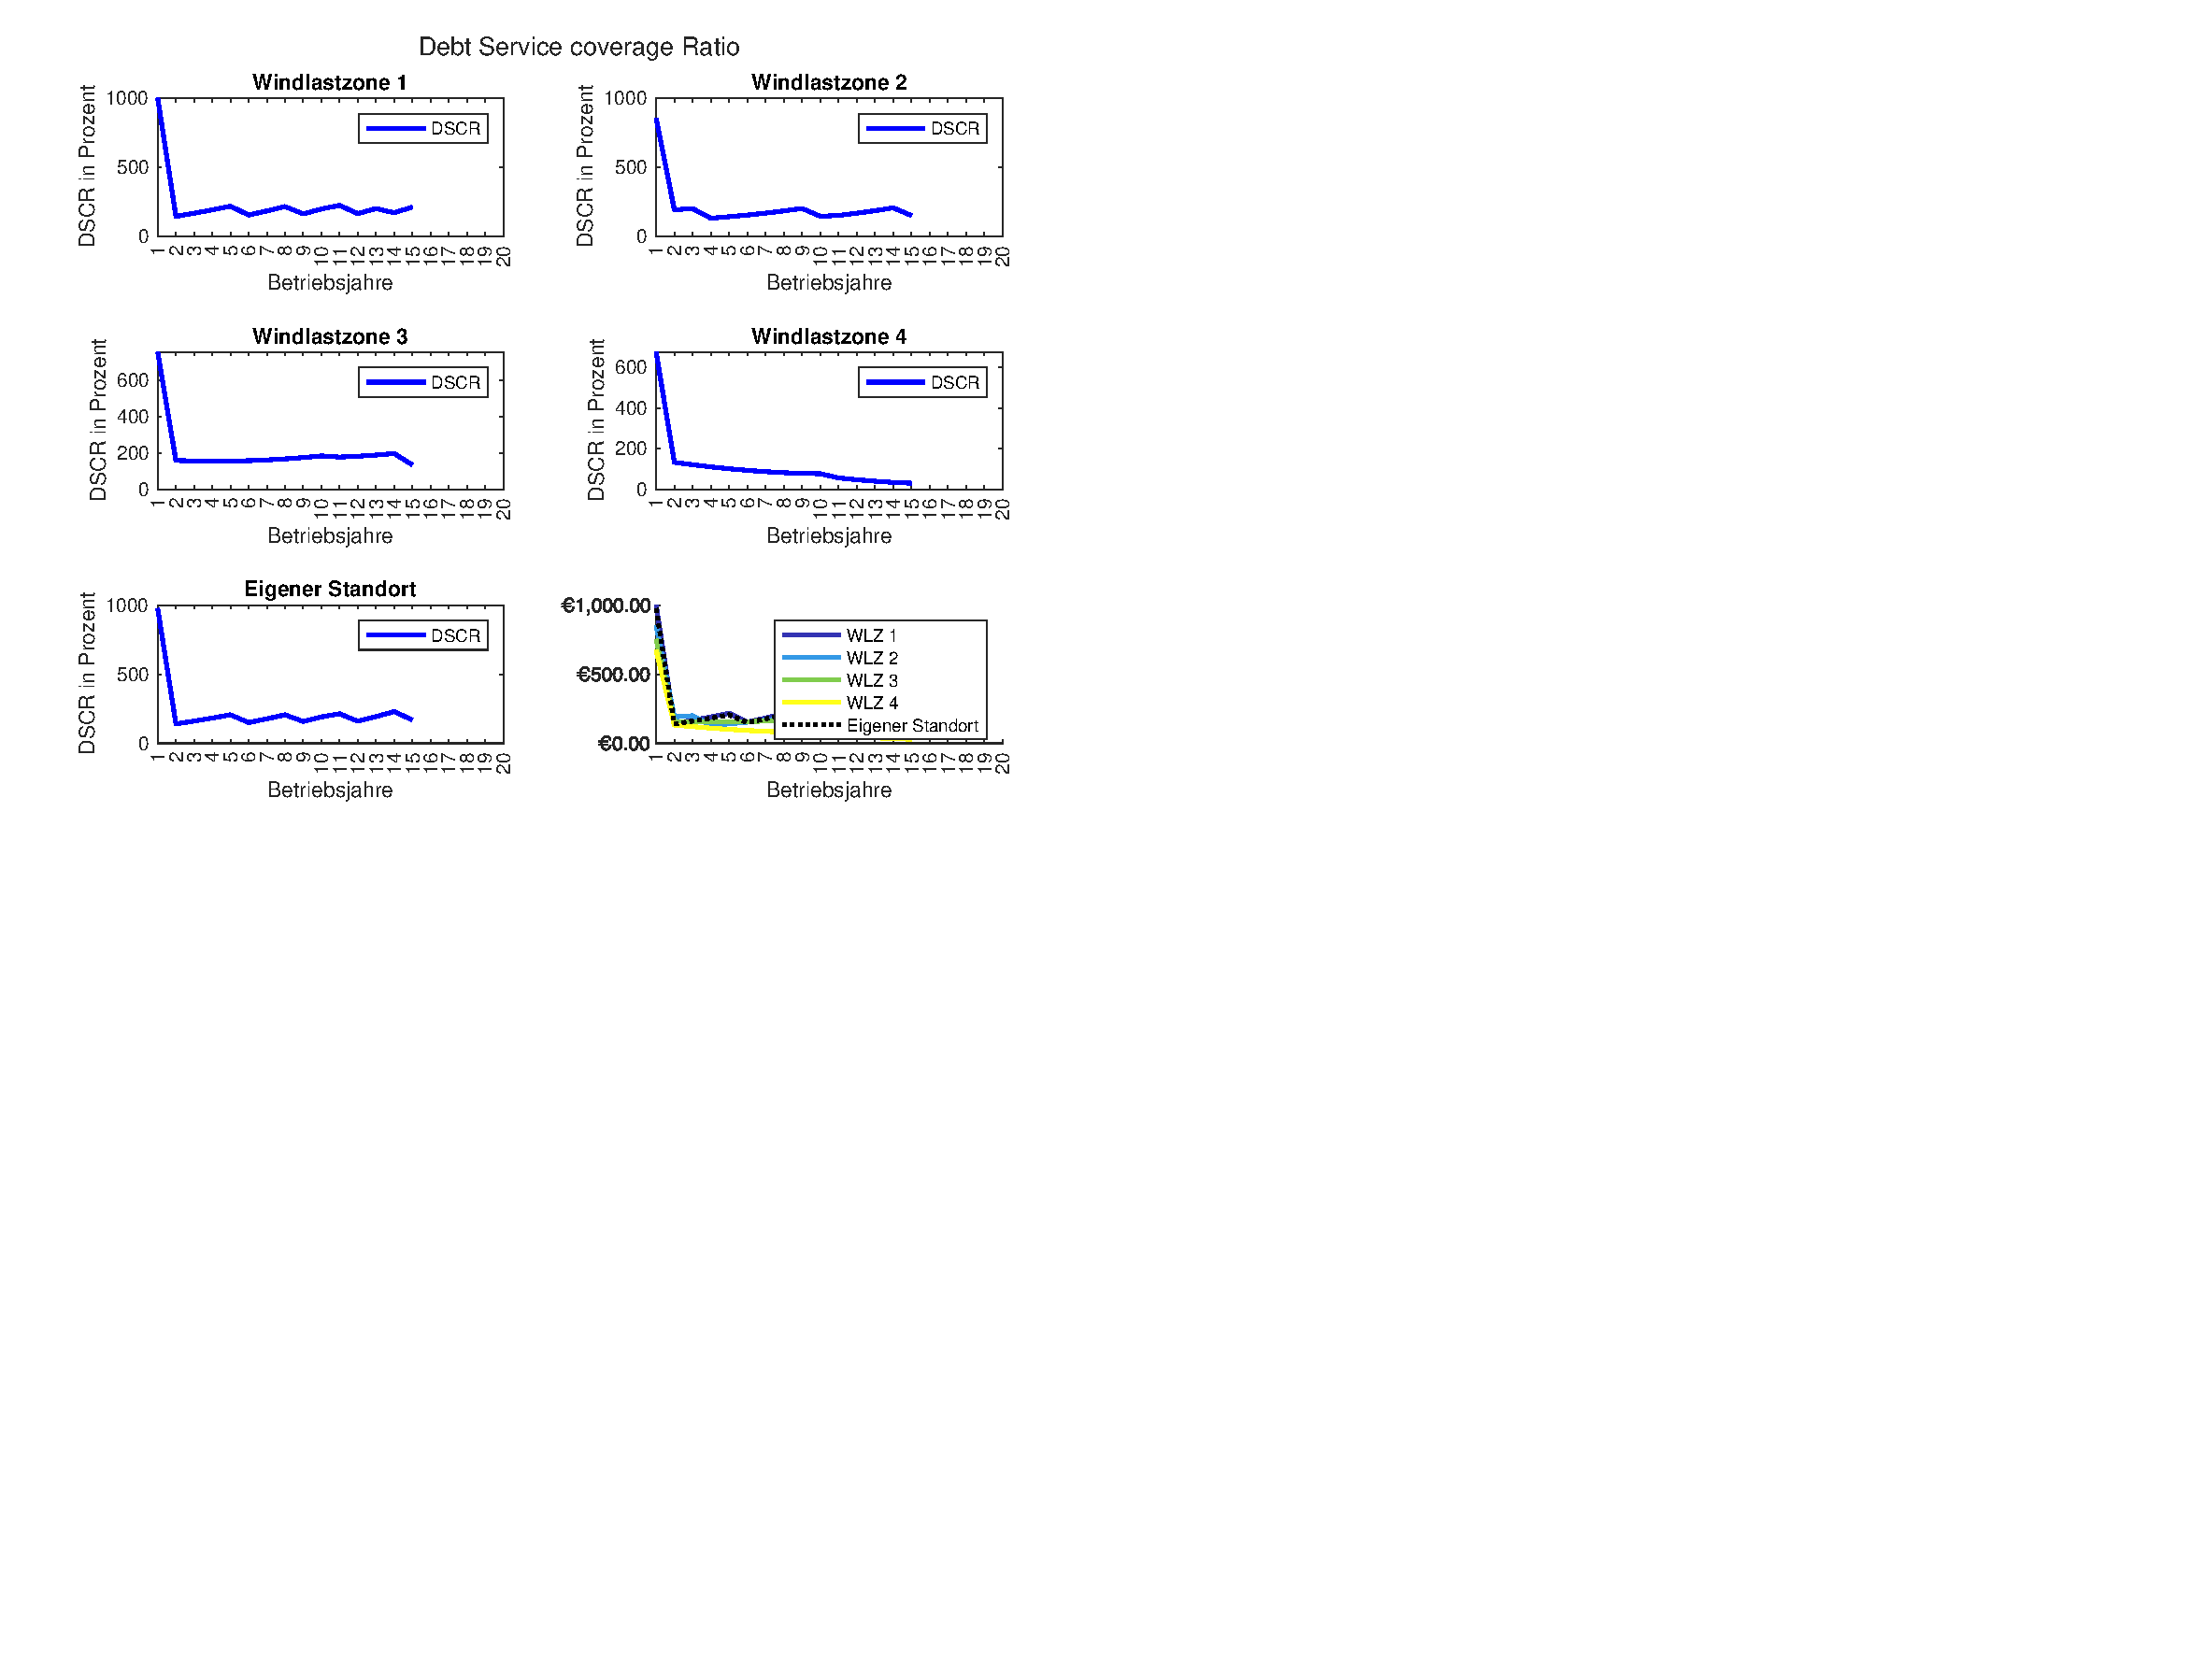
\includegraphics[width=\maxwidth{56.196688409433015em}]{figure_1.eps}
\end{center}
\end{document}
